\documentclass[12pt,answers]{exam}
\usepackage{amsmath,amsfonts,amssymb,commath,mathtools,physics}
\usepackage{todonotes}
\usepackage{enumitem}
\usepackage{float}
\newcommand{\vect}[1]{\left\langle #1 \right\rangle}
\newcommand{\tcurl}{\operatorname{curl}}
\newcommand{\tdiv}{\operatorname{div}}
\newcommand{\tgrad}{\operatorname{grad}}
\newcommand{\RR}{\mathbb{R}}

\pagestyle{headandfoot}
\firstpageheadrule
\runningheadrule
\firstpageheader{Math 222}{Final Exam Makeup|Solutions, Page \thepage\ of \numpages}{2018 Fall}
\runningheader{Math 222}{Final Exam Makeup|Solutions, Page \thepage\ of \numpages}{2018 Fall}
\runningfooter{}{}{}

% \title{2018 Fall Calc 3 Final Version A|Solutions}
% \author{Winston Cheong}
% \date{}

\begin{document}
% \maketitle
\begin{questions}
  \question Here is a vector which you can assume has unit length:
  \begin{figure}[H]
    \centering
    \vspace{.5in}
    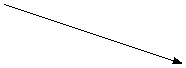
\includegraphics{graphics/2018-fall-final-vb-1.pdf}
    \vspace{.5in}
  \end{figure}
  Call this vector $\vb{u}$. Now using the same base point draw a vector $\vb{w}$ (and label it) so that the following are all satisfied:
  \begin{enumerate}[label=(\alph*)]
    \item $|\vb{w}| = 1$.
    \item $\vb{u} \cross \vb{w}$ points away from you
    \item $\vb{u} \cross \vb{w} \approx 1/2$. (Try to make it as close as you can.)
  \end{enumerate}
  Next using the same base point again draw a vector $\vb{v}$ (and label it) so that the following are all satisfied:
  \begin{enumerate}[label=(\alph*)]
    \item $|\vb{v}| = 1$.
    \item $\vb{u} \vdot \vb{v} \approx 1/2$. (Again, do your best to get equality.)
    \item $\vb{u} \cross \vb v$ points toward you.
  \end{enumerate}
  \begin{solution}
    
    \begin{align*}
      \vb u \cross \vb w &= \| \vb u \| \|\vb w\| \sin \theta = \frac12 \implies \theta = 30^\circ \\ 
      \vb u \vdot \vb v &= \| \vb u \| \|\vb v\| \cos \theta = 1/2 \implies \theta = 60^\circ
    \end{align*}
    so the final configuration looks like
    \begin{figure}[H]
      \centering
      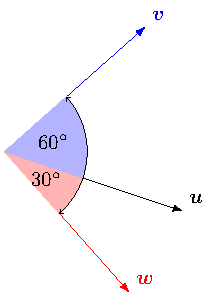
\includegraphics{graphics/2018-fall-final-vm-1-sol.pdf}
    \end{figure}
  \end{solution}
  
  \newpage
  \question
  Short answers\ldots Intuition and Understanding
  \begin{parts}
    \part If you are driving, then what device (or devices) in your car will be the best way to change your normal acceleration?
    \begin{solution}
      Steering wheel
    \end{solution}
    
    \part What is the curvature of a circle with radius 25?
    \begin{solution}
      $\kappa = \frac{1}{25}$
    \end{solution}
    
    \part $f(x,y)$ is defined to equal 3 for all points on the disk $(x-1)^2 + (y-2)^2 \le 4$, to equal $-2$ for all points on the disk $(x+4)^2 + (y+7)^2 \le 9$, and to equal 0 everywhere else. Compute:
    \[
    \int_{x=-90}^{100} \int_{y=-100}^{90} f(x,y) \dif y \dif x.
    \]
    \begin{solution}
      $= 3 \cdot \pi (2^2) - 2 \pi (3^2) = \boxed{-6\pi}$
    \end{solution}
    
    \part Will the surface integral
    \[
    \iint_{S} f(x,y,z) \dif S
    \]
    typically give you the surface area of $S$? Explain your answer in one sentence or less.
    \begin{solution}
      No. Only if $f(x,y,z) = 1$ will the integral compute the surface area of $S$.
    \end{solution}
    \part What is the average value of the function $f(x,y) = 1 + 2x$ on the rectangle $1\le x \le 5$, $3 \le y \le 6$?
    \begin{solution}
      \[
      = \frac{\int_3^6 \int_1^5 (1+2x) \dif x \dif y}{(5-1)(6-3)}
      = \frac{\int_3^6 1 \dif y \cdot \int_1^5 (1+2x) \dif x}{12}
      = \frac{3\left[x+x^2\right]_1^5}{12}
      =\frac{3\cdot 28}{12}
      = \boxed{7}
      \]
    \end{solution}
  \end{parts}
  
  \newpage
  \question
  Short answers\dots Definitions and Theorems
  \begin{parts}
    \part Suppose that $\nabla f(0,0) = \vect{0,0}$, and $f_{xx}(0,0)$ and $f_{yy}(0,0)$ are both positive. Do you need anything else to conclude that $(0,0)$ is a local minimum? (If yes, then what? If no, then why not?)
    \begin{solution}
      Yes, need to know that the discriminant $> 0$.
      In particular, that $f_{xx}(0,0) f_{yy}(0,0) > f_{x,y}(0,0)^2$.
    \end{solution}
    \part What does it mean (definition!) for a vector field $\vb{F}(x,y,z)$ to be incompressible?
    \begin{solution}
      $\tdiv \vb{F} = 0$.
    \end{solution}
    \part According to the theorem that we learned, if $f$ is a continuous function on a set $\Omega$, then what condition or conditions on $\Omega$ will guarantee that $f$ attains an absolute maximum and absolute minimum?
    \begin{solution}
      $\Omega$ must be closed and bounded
    \end{solution}
    \part Assume that you have been given a differentiable vector field defined on the first octant. How can you quickly tell if it is conservative?
    \begin{solution}
      Since it is defined on the entire first octant (a simply connected domain), the vector field is conservative if and only if its curl is the zero vector.
    \end{solution}
  \end{parts}
  
  \newpage
  \question
  A certain differentiable function satisfies:
  \begin{enumerate}[label=(\alph*)]
    \item $f(9,7) = 1$, and $f(2,-4)= 6$
    \item $\nabla f(9,7) = (5,3)$, and $\nabla f = (2,-4) = (-\pi,8)$.
  \end{enumerate}
  At each of the two points in question (i.e.~at $(9,7)$ and at $(2,-4)$) answer the following questions:
  \begin{parts}
    \part In what direction is the function increasing the fastest?
    \begin{solution}~\\
      For $(9,7)$: $\vect{5, 3}$; \\
      For $(2,-4)$: $\vect{-\pi, 8}$.
    \end{solution}
    
    \part What is the rate of change in that direction?
    \begin{solution}~\\
      For $(9,7)$: $\sqrt{25 + 9} = \sqrt{34}$; \\
      For $(2,-4)$: $\sqrt{\pi^2+64}$.
    \end{solution}
    
    \part What is the directional derivative in the direction of $\vect{3,-4}$? (Note: just to be completely clear about semantics here, you are supposed to give the same directional derivative at each point. I did not ask for the directional derivative in the direction of the point $(3,-4)$.)
    \begin{solution}
      Let $\vb u = \vect{\frac35, -\frac45}$.
      
      For $(9,7)$: $D_{\vb u} f(9,7) = \nabla f(9,7) \vdot \vb{u} = \vect{5,3} \vdot \vect{\frac35, -\frac45} = \frac{3}{5}$. \\
      For $(2,-4)$: $D_{\vb u} f(2,-4) = \nabla f(2,-4) \vdot \vb{u} = \vect{-\pi,8} \vdot \vect{\frac35, -\frac45} = \frac{-32-3\pi}{5}$.
    \end{solution}
    
    \part What is the tangent plane and/or the linear approximation at each of the two points?
    \begin{solution}~\\
      For $(9,2)$: $L(x, y) = 1 + 5(x-9) + 3(y- 7)$\\
      For $(-2,4)$: $L(x, y) = 7 - \pi(x+2) + 8(y - 4)$
    \end{solution}
  \end{parts}
  
  \newpage
  \question
  Find the maximum and minimum of the function
  \[
  f(x,y) = 8x^2-4x+\frac{y^2}{3}
  \]
  on the set 
  \[
  g(x,y) = 4x^2 + \frac{y^2}{9} \le 4.
  \]
  Show your work carefully, and explain what you are doing. (No essays, please. Just a few short words in the right places will suffice.)
  \begin{solution}
    First, consider $g < 4$. Setting $\nabla f = 0$, and solving
    \[
    \nabla f = \vect{16x-4,\frac23 y} = \vb 0
    \]
    gives the critical point $(\frac14, 0)$.
    Next, considering $g = 4$, we solve $\nabla f = \lambda \nabla g$:
    \[
    \left\{
    \begin{aligned}
      16x-4&=8\lambda x\\
      \frac23y&=\frac29\lambda y\\
      4x^2 + \frac{y^2}{9} &= 4
    \end{aligned}
    \right.
    \]
    Solving this system gives 
    four constrained critical points: $(1,0)$, $(-1, 0)$, $(-\frac12, 3\sqrt 3)$, $(-\frac12, -3\sqrt 3)$
    Evaluating $f$ on the found critical points:
    \begin{align*}
      f(\frac14, 0) &= -\frac12 \\ 
      f(1,0) &= 4 \\
      f(-1, 0) &= 12 \\ 
      f(-\frac12, 3\sqrt 3) &= 13 \\
      f(-\frac12, -3\sqrt 3) &= 13
    \end{align*}
    Thus the maximum is $13$, and the minimum is $-\frac1{2}$.
  \end{solution}
  
  \newpage
  \question
  Let $S$ be the part of the set 
  \[
  z = \sqrt{x^2 + y^2}
  \]
  which is between the planes $z=2$ and $z=5$ and which has $x \ge 0$. \\ 
  Express the surface area for $S$ as an iterated integral (i.e.~a double or triple integral) over a subset of $\RR^2$ or $\RR^3$ which has \textbf{constant} bounds of integration. (i.e.~it should be over a rectangular solid or a rectangle in the domain in which you are finally integrating.) You do \textbf{NOT} need to find this integral.
  \begin{solution}
    The set $S$ can be parametrized by 
    \[
    G(r, \theta) = (r\cos \theta, r\sin\theta, r) 
    \qquad 2 \le r \le 5, 
    \quad 0 \le \theta \le 2\pi
    \]
    We can then compute
    \begin{align*}
      \vb{N} = G_r \cross G_\theta 
      &= \vect{\cos \theta, \sin\theta, 1} \cross \vect{-r\sin\theta, r\cos\theta, 0}  \\ 
      &= \vect{-r\cos\theta, -r\sin\theta, r}
    \end{align*}
    and
    \[
    \|\vb{N}\| = \sqrt{r^2\cos^2\theta+r^2\sin^2\theta+r^2} = \sqrt{2r^2} = r\sqrt 2
    \]
    The surface area of $S$ can thus be computed as the surface integral
    \[
    \iint_S 1 \dif S  = \boxed{\int_{-\frac\pi2}^{\frac\pi2} \int_2^5 r \sqrt 2 \dif r \dif \theta}
    \]
  \end{solution}
  
  \newpage
  \question
  Let $C$ be the curve given by
  \[
  \vb{r}(t) = \left(
    1+\sin^2(2t),
    \sin^2(2t)
  \right),
  \]
  with $0 \le t \le \pi/4$. Compute the following integral:
  \[
  \int_C \vect{2x+\pi \cos(\pi x)e^{2y}, 3y^2+2\sin(\pi x)e^{2y}} \vdot \dif \vb{r}.
  \]
  \begin{solution}
    The vector field above has potential function $f = x^2 + \sin(\pi x)e^{2y} + y^3$, so the line integral is over a conservative vector field.
    Hence by the Fundamental Theorem for Line Integrals,
    \begin{align*}
      \int_C \vb{F} \vdot \dif \vb{r}
      & = f(\vb{r}(\pi/4)) - f(\vb{r}(0)) \\
      & = f(2,1) - f(1,0)   \\
      & = (4+0+1) - (1+0+0)
      = \boxed{4}
    \end{align*}
  \end{solution}
  
  \newpage
  \question
  Let $Q$ be the set of points within the set:
  \[
  \{ (x,y,z) : x^2+y^2+z^2 \le 4, \quad \text{and } 0 \le y \}
  \]
  and let $\partial Q$ be the boundary of this set. If $\vb{n}$ is the outward unit normal to this region, then compute:
  \[
  \iint_{\partial Q} (ze^{3y}, y^2, y\sin(2y)) \vdot \vb{n} \dif S.
  \]
  \begin{solution}
    The set $Q$ is the right hemisphere of a ball of radius 2.
    The divergence theorem, states that
    \[
    \iint_{\partial Q} \vb{F} \vdot \dif \vb{S} = \iiint_{Q} \tdiv \vb F \dif V
    \]
    For the vector field above, we have $\tdiv \vb F = 0 + 2y + 0 = 2y$
    so 

    \begin{align*}
      \iint_{\partial Q} \vb F \vdot \vb{n} \dif S
      &= \iiint_Q 2y \dif V
    \end{align*}
    Evaluating this integral in spherical coordinates,
    \begin{align*}
      \iiint_{Q} 2y \dif V 
      &= \int_{0}^{\pi} \int_0^\pi \int_0^2 2 \rho \sin\varphi \sin\theta \cdot \rho^2 \sin\varphi \dif \rho \dif \varphi \dif \theta\\
      &= \int_0^2 2\rho^3 \dif \rho 
      \cdot
      \int_{0}^{\pi} \sin\theta \dif \theta
      \cdot
      \int_0^\pi \sin^2\varphi \dif \varphi 
      \\
      &= \left[ \frac{\rho^4}{2} \right]_0^2
      \cdot
      \left[-\cos\theta\right]_0^\pi
      \cdot
      \left[\frac12 \varphi - \frac14 \sin2\varphi\right]_0^\pi
      \\
      &= 8 \cdot (1+1) \cdot (\frac\pi2 - 0 - 0) 
      \\
      &= \boxed{8\pi}
    \end{align*}
  \end{solution}
  
  \newpage
  \question
  Let $E$ be the subset of
  \[
  z = x^2 + y^2
  \]
  which also satisfies 
  \[
  z \le 49, \qquad x \le 0, \qand y \ge 0.
  \]
  Express
  \[
  \iint_E (x^2 + y^3) \dif S
  \]
  as an iterated integral (i.e.~a double or triple integral) over a subset of $\RR^2$ or $\RR^3$. You do \textbf{NOT} need to find this integral.
  \begin{solution}
    The set $E$ can be parametrized by 
    \[
    G(r, \theta) = (r \cos \theta, r\sin\theta, r^2) 
    \qquad 0 \le r \le 7, 
    \quad \frac\pi2\le \theta \le \pi
    \]
    Then we can compute
    \begin{align*}
      \vb{N} = G_r \cross G_\theta 
      &= \vect{\cos \theta, \sin\theta, 2r} \cross \vect{-r\sin\theta, r\cos\theta, 0}  \\ 
      &= \vect{-2r^2\cos\theta, -2r^2\sin\theta, r}
    \end{align*}
    and
    \[
    \|\vb{N}\| = \sqrt{4r^4+r^2}
    \]
    Which allows to rewrite the integral as
    \[
    \iint_E (x^2+y^3) \dif S 
    = \boxed{\int_{\frac\pi2}^\pi \int_0^7 (r^2 \cos^2\theta + r^3\sin^3\theta) \cdot \sqrt{4r^4+r^2} \dif r \dif \theta}
    \]
    
  \end{solution}
  
  \newpage
  \question
  Let $E$ be the part of the set
  \[
  x^2+y^2 \le z \le 4
  \]
  that also satisfies
  \[
  x \le 0 \qand y \le 0.
  \]
  Express
  \[
  \iiint_{E} (2x + 3y) \dif V.
  \]
  \begin{solution}
    The inequality can be reexpressed as 
    $0 \le r^2 \le z \le 4$. 
    The bounds for the variables are
    \[
    \theta \in [\pi, \frac{3\pi}{2}] 
    \qquad 
    r \in [0,2]
    \qquad
    z \in [r^2,4]
    \]
    $E$ is a quarter of a solid cone.
    The integral can be written in cylindrical coordinates as
    \[
    \iiint_E(2x+3y) \dif V
    = \boxed{\int_\pi^{\frac{3\pi}{2}} \int_0^2 \int_{r^2}^4 (2r\cos\theta+3r\sin\theta) \cdot r \dif z \dif r \dif \theta }
    \]
  \end{solution}
  
\end{questions}

\end{document}
